\chapter{背景}
\label{chap:background}
本章では本研究の背景となった、
モバイルデバイスへの文字入力機会増加、日本語入力と英語入力の差異、
日本語IMEの不満について述べる。
について述べる。

\newpage
\section{モバイルデバイスへの文字入力の機会の増加}
今日モバイルデバイスにおいて、文字入力をする機会が増加している。
そのためIMEの省入力化への需要が高まっている。
それにはいくつかの要因があり、
そのいくつかの要因についてここでは論ずる。

\subsection{モバイルデバイスの普及}
現在、日本において
スマートフォンやタブレットなどのモバイルデバイスが大幅かつ急激に普及した。
総務省による「平成25年通信利用動向調査」
\cite{communicationreport}の
「通信端末世帯保有率の推移」
(図:\ref{fig:mobiledevicespread})によると、
\begin{figure}[htbp]
  \begin{center}
    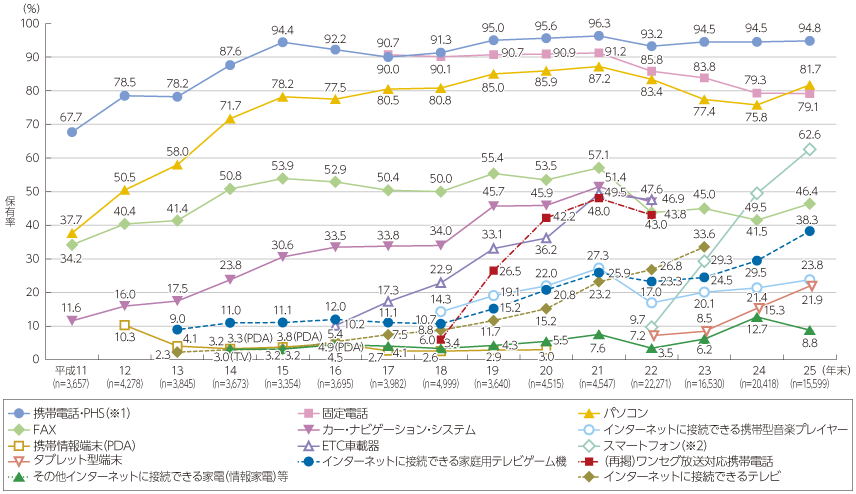
\includegraphics[width=160mm,bb=0 0 856 494]{images/mobiledevicespread.png}
    \caption{情報通信端末世帯保有率の推移(出典:\cite{communicationreport})}
    \label{fig:mobiledevicespread}
  \end{center}
\end{figure}
平成22年には9.7%しかなかったスマートフォンの普及率は、
平成25年には62.6%と急激に成長している。
平成22年から平成25年の3年間で52.9%の伸びを見せており、
これはパソコンの保有率が最も伸びた平成11年から平成14年の
伸び率を大きく上回る数字となっている。
このデータからもスマートフォンの普及はいまだかつてないほどの
速度で進行していることがわかる。
本論文においてはスマートフォンとは多機能なモバイルデバイスであり
パソコンとしての機能を果たすことができるものを意味していて、
具体的にはAndroidOS
\footnote{http://www.google.com/intl/ja/mobile/android/}
,iOS\footnote{http://www.apple.com/jp/ios/}
などを搭載しているものである。
またタブレットとはスマートフォンと同じ要件を満たしながら、
画面の大きさがスマートフォンよりより大きい物を意味している。

\subsection{モバイルデバイスの用途}
ユーザーはスマートフォンを使うことではパソコンと同様に多くのことができる。
その中でもスマートフォンユーザーは
文字入力を行う可能性が高いアプリケーションを頻繁に使用している。
リサーチバンクによるアンケート調査\cite{researchbanksmartphone}
(図:\ref{fig:purpose})によると
\begin{figure}[htbp]
  \begin{center}
    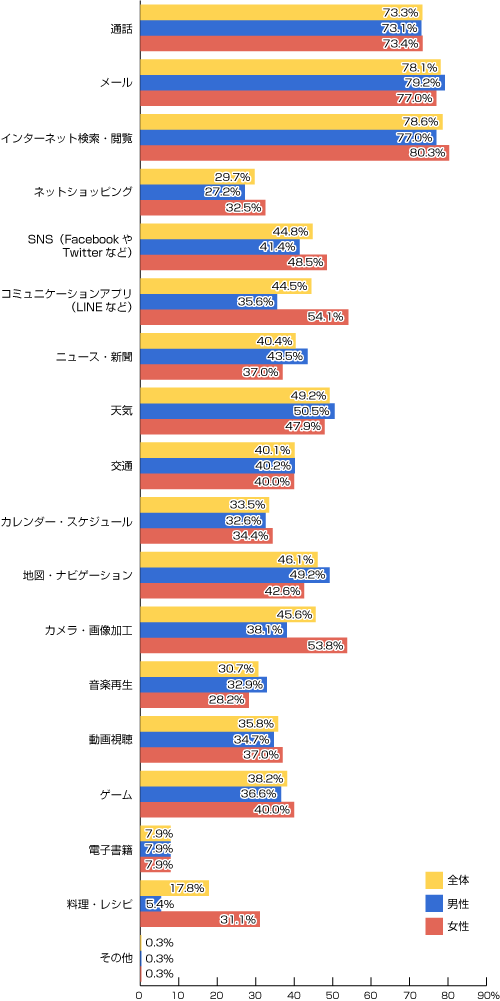
\includegraphics[width=115mm,bb=0 0 500 1001]{images/purpose.png}
    \caption{スマートフォンでどのような機能・アプリを使っているか(出典:\cite{researchbanksmartphone})}
    \label{fig:purpose}
  \end{center}
\end{figure}
メールアプリを使う人が78.1%、SNSアプリを使う人が44.8%、
コミュニケーションアプリを使う人が44.5%となっている。
メールアプリ、コミュニケーションアプリ、SNSアプリはそれぞれ
スマートフォンを
情報の受信端末としてのみ使う場合には文字入力の必要はないが、
情報を発信しようとする場合には文字入力が必要である。
スマートフォンにおける他のアプリケーション
においても適時文字入力が必要である。
こういった結果から
スマートフォンを使うユーザーは文字入力の機会がとても多いことがわかる。

\subsection{デバイスの多様化}
デバイスが多様化し、文字入力の機会が増えている。
スマートウォッチ(図:\ref{fig:smartwatch})や、
ヘッドマウントディスプレイの一つである
Google Glass(図:\ref{fig:googleglass})がその例として挙げられる。
\begin{figure}[htbp]
  \begin{minipage}{0.5\hsize}
    \begin{center}
      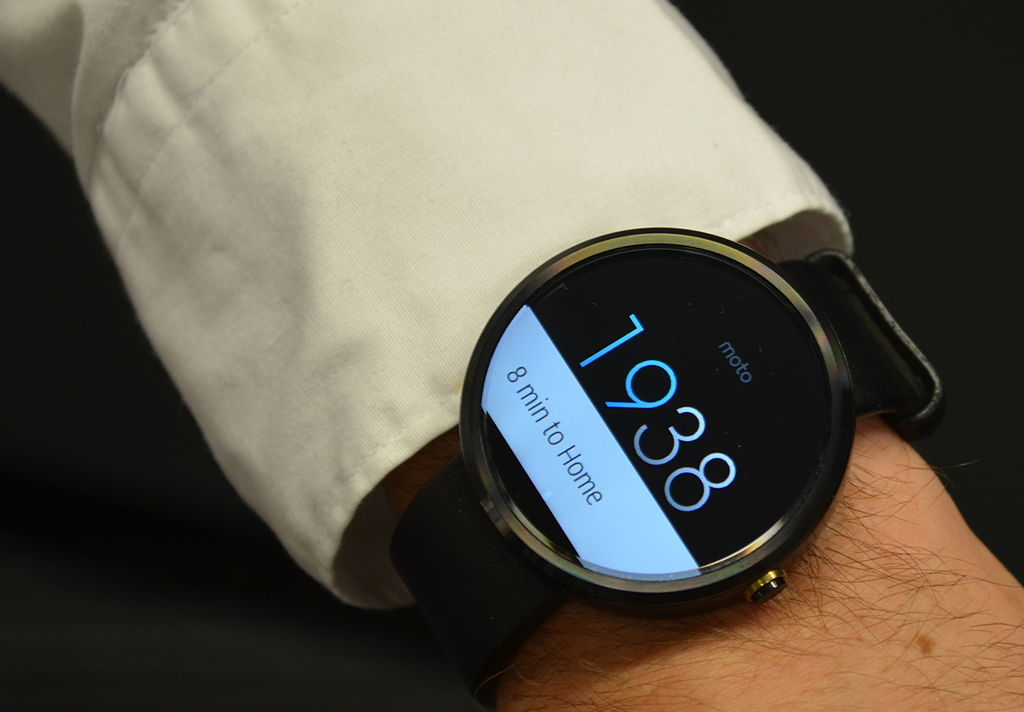
\includegraphics[width=70mm,bb=0 0 246 171]{images/smartwatch.png}
    \end{center}
    \caption{スマートウォッチの例:Android Wearを搭載したMoto360(出典:\cite{smartwatch})}
    \label{fig:smartwatch}
  \end{minipage}
  \begin{minipage}{0.5\hsize}
    \begin{center}
      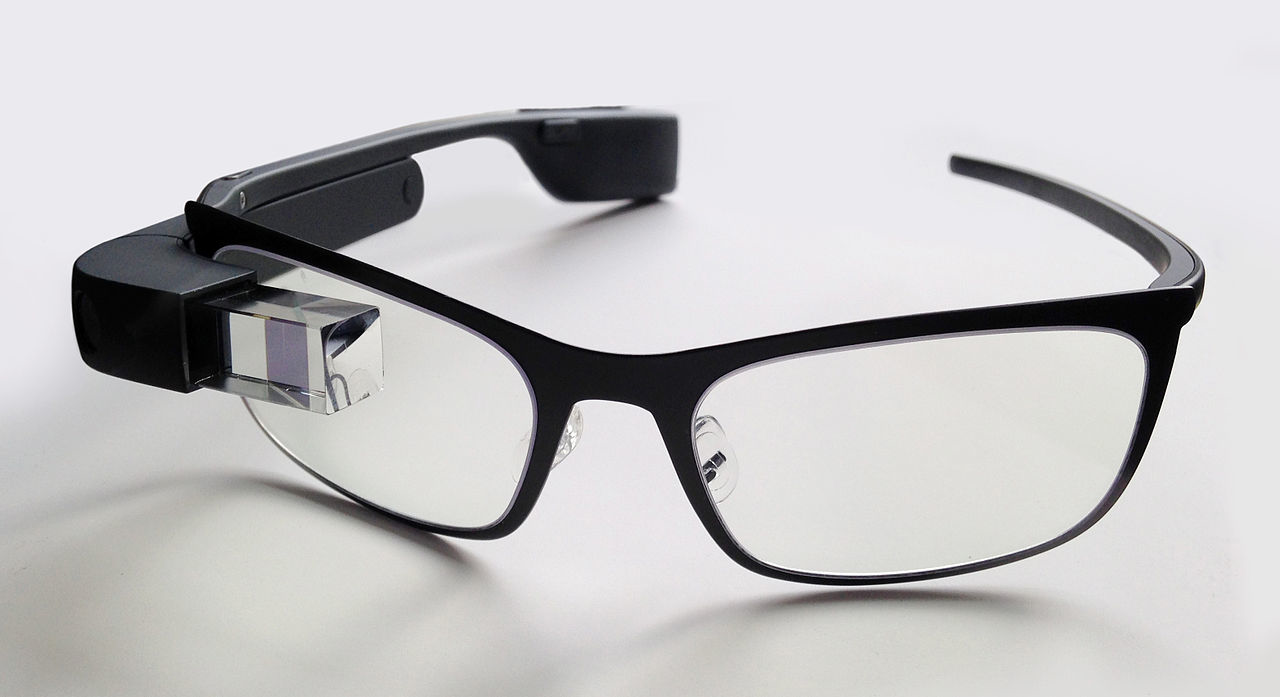
\includegraphics[width=70mm,bb=0 0 1280 697]{images/googleglass.png}
    \end{center}
    \caption{Google glass(出典:\cite{googleglass})}
    \label{fig:googleglass}
  \end{minipage}
\end{figure}
スマートウォッチは既存の時計にモバイルデバイス向けOSを搭載したもので、
従来の時計であれば文字入力とは無縁であったが、
これを使うことで文字入力をこのデバイス上でも
行う必要が出てくる。
Google glassにおいても同様でメガネにおいて必要のなかった文字入力が
こういったデバイスになることで文字入力が必要となる。

\section{日本語入力と英語入力の差異}
日本語と英語ではコンピューターに対する入力にかかるコストが大きく異なる。
qwertyキーボードで日本語を入力する場合、
アルファベットを入力しそれをひらがなに日本語IMEが変換し、
それを漢字やカタカナの混ざった文章に変換するというプロセスになる。
英語においては入力したアルファベットがそのまま文章となるため、
IMEを使う必要がなく、ほとんど使われていないのが現状である。
このため英語圏においていままで研究が盛んではなく、
世界中でのIMEやそれに対する研究の需要は増している。

\section{入力システムの変遷}
現在どのようなOSを使用しているスマートフォンであって
も必ずIMEアプリケーションは搭載されている。
これらのモバイルデバイスを使用する上で
日本語の入力は欠かすことができない操作である。
デバイスの性能は携帯電話の頃から劇的に向上している。
今日ではパソコンに遜色のないような
CPUやメモリを積んでいるものも多く市販されている。
デバイスの性能が向上している間に
様々なテキスト入力方式などが考案された\cite{増井俊之:2002-08-01}
が搭載されている入力方式には携帯電話の時から大きな変化はない。
日本語IMEにおける内部的なシステムとしては、
連文節変換や予測入力システム\cite{pobox}
が開発され、IMEへの導入がおこなわれた。
これらのシステムは様々に応用可能で広く
普及したがいまだ日本語IMEへの改善の余地は多く残されていると考える。

\section{日本語IMEへの不満と期待}
日本語IMEには様々な不満と期待が存在する。

\subsection{日本語IMEへの不満}
楽天リサーチによる「スマートフォンに関する調査」
(出典:\cite{rakutensmartphone})によると、
スマートフォンを使うユーザーが挙げる不満点の中で
最も割合が大きいのが「文字入力がしにくい」ということである。
(スマートフォンを利用している際に不便だと感じる点 出典:\cite{rakutensmartphone})
\begin{figure}[htbp]
  \begin{center}
    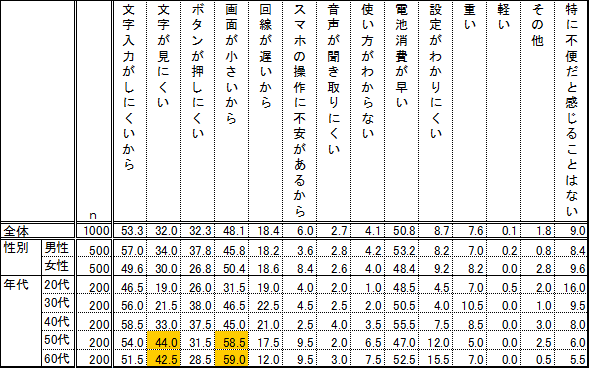
\includegraphics[width=140mm,bb=0 0 589 368]{images/dissatisfaction.png}
    \caption{スマートフォンを利用している際に不便だと感じる点(出典:\cite{rakutensmartphone})}
    \label{fig:dissatisfaction}
  \end{center}
\end{figure}
文字入力がしにくい理由としてはデバイスが携帯電話から
変化しているにもかかわらず、
IMEの入力方式インタフェースがほとんど変わっていないためであると考えた。
携帯電話の時には折りたたみ式やストレート式、スライド式といくつか存在したが、
\begin{figure}[htbp]
  \begin{minipage}{0.3\hsize}
    \begin{center}
      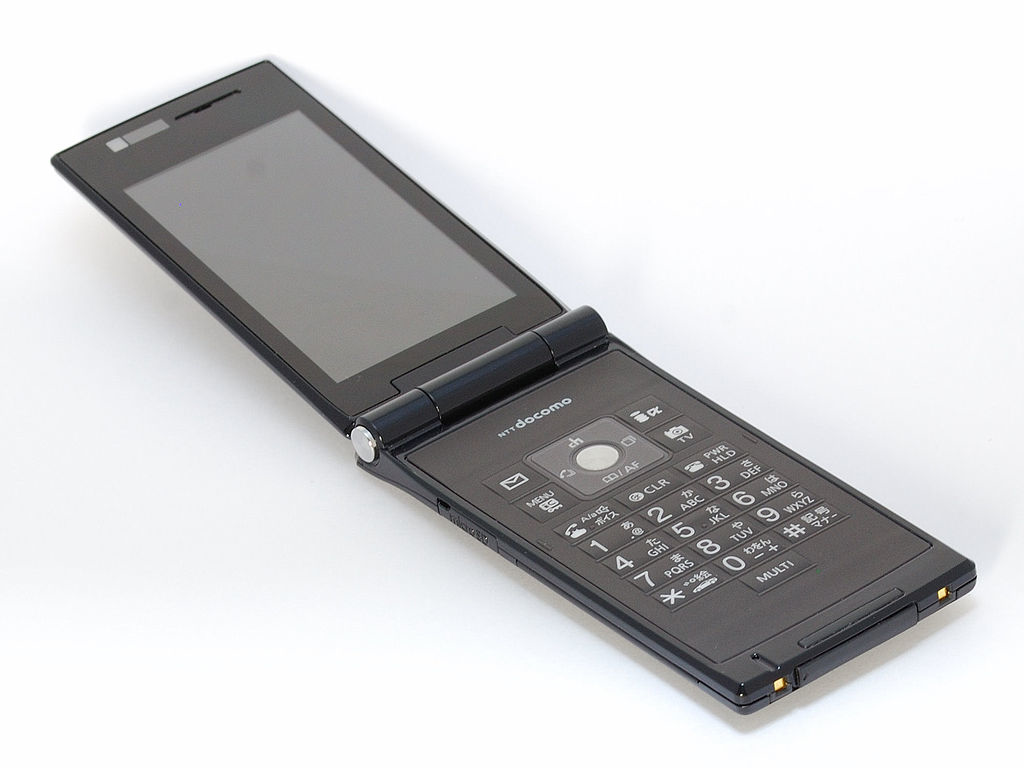
\includegraphics[width=50mm,bb=0 0 1024 768]{images/oritatami.png}
    \end{center}
    \caption{折りたたみ式携帯電話例:(出典:\cite{keitai})}
    \label{fig:oritatami}
  \end{minipage}
  \begin{minipage}{0.3\hsize}
    \begin{center}
      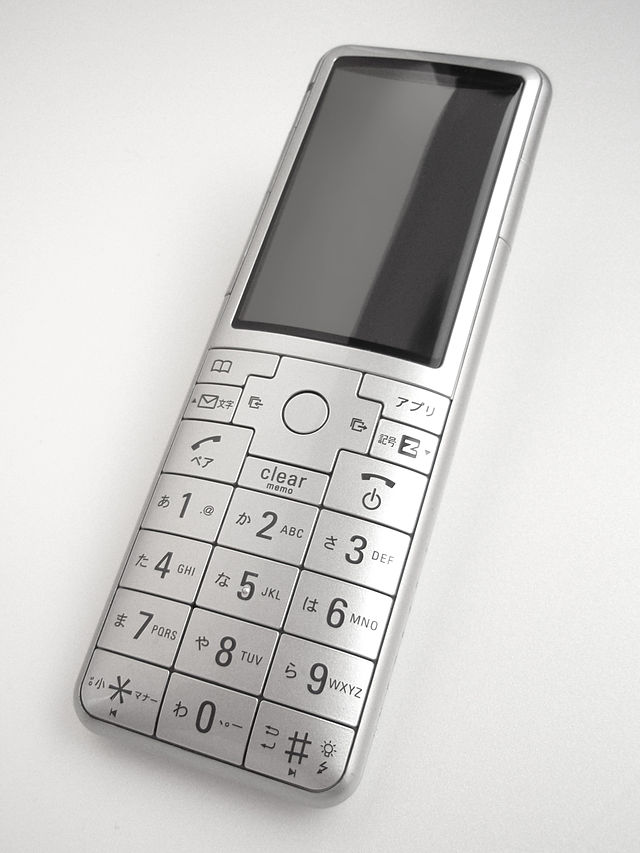
\includegraphics[width=50mm,bb=0 0 147 196]{images/straight.png}
    \end{center}
    \caption{ストレート式携帯電話例(出典:\cite{keitai})}
    \label{fig:straight}
  \end{minipage}
  \begin{minipage}{0.3\hsize}
    \begin{center}
      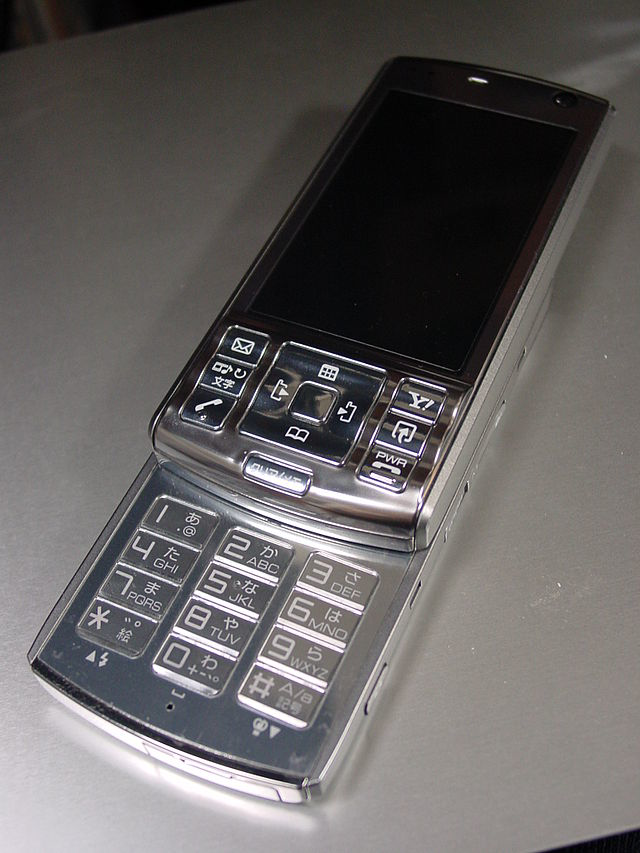
\includegraphics[width=50mm,bb=0 0 154 205]{images/slide.png}
    \end{center}
    \caption{スライド式携帯電話例:(出典:\cite{keitai})}
    \label{fig:slide}
  \end{minipage}
\end{figure}
入力方式はどれもキーパッド式であり、12個あるキー
(あかさたなはまやらわ\#*)をそれぞれ
何度も押すことで、(三回タッチすると「あ→い→う」の用に変化する)
文字を入力していく方式であった。
しかし現在のモバイルデバイスは多くがタッチスクリーン式
に変化しており、これらキーパッド方式時代の名残である
入力方式はタッチスクリーンでの体験を重視したものに
変化させていくべきである。\cite{designinginterface}

\subsection{IMEへの期待}
最終的には入力したいと思った文字を何もせずにそのまま
入力できるようなIMEを開発したいと考えている。
しかしそこまでにはまだまだ現状とは大きな隔たりがある。
そこでその前段階としてコンテキストからユーザーの
入力したい単語を推測し、提示することで
入力のユーザーエクスペリエンスを大幅に向上させるIME
を研究・開発した。
また今回は日本語IMEとして実装したが、
実装されているコンテキスト推薦機能などは
